\chapter{Améliorations du développement logiciel : }
    \section{Des outils de détection classique : quel point de départ ?}
        %citer 1, 2, 17, 46
        \subsection{Détection de vulnérabilités par IA : un bref état de l'art}
            \subsubsection{Copilot : brève analyse de l'existant}
            \subsubsection{Tabnine : un exemple de standard industriel pour la sécurisation de code par IA}
                %46
        \subsection{Cas particulier du code généré par des LLM}
                \begin{figure}[H]
                    \centering
                    {\fbox{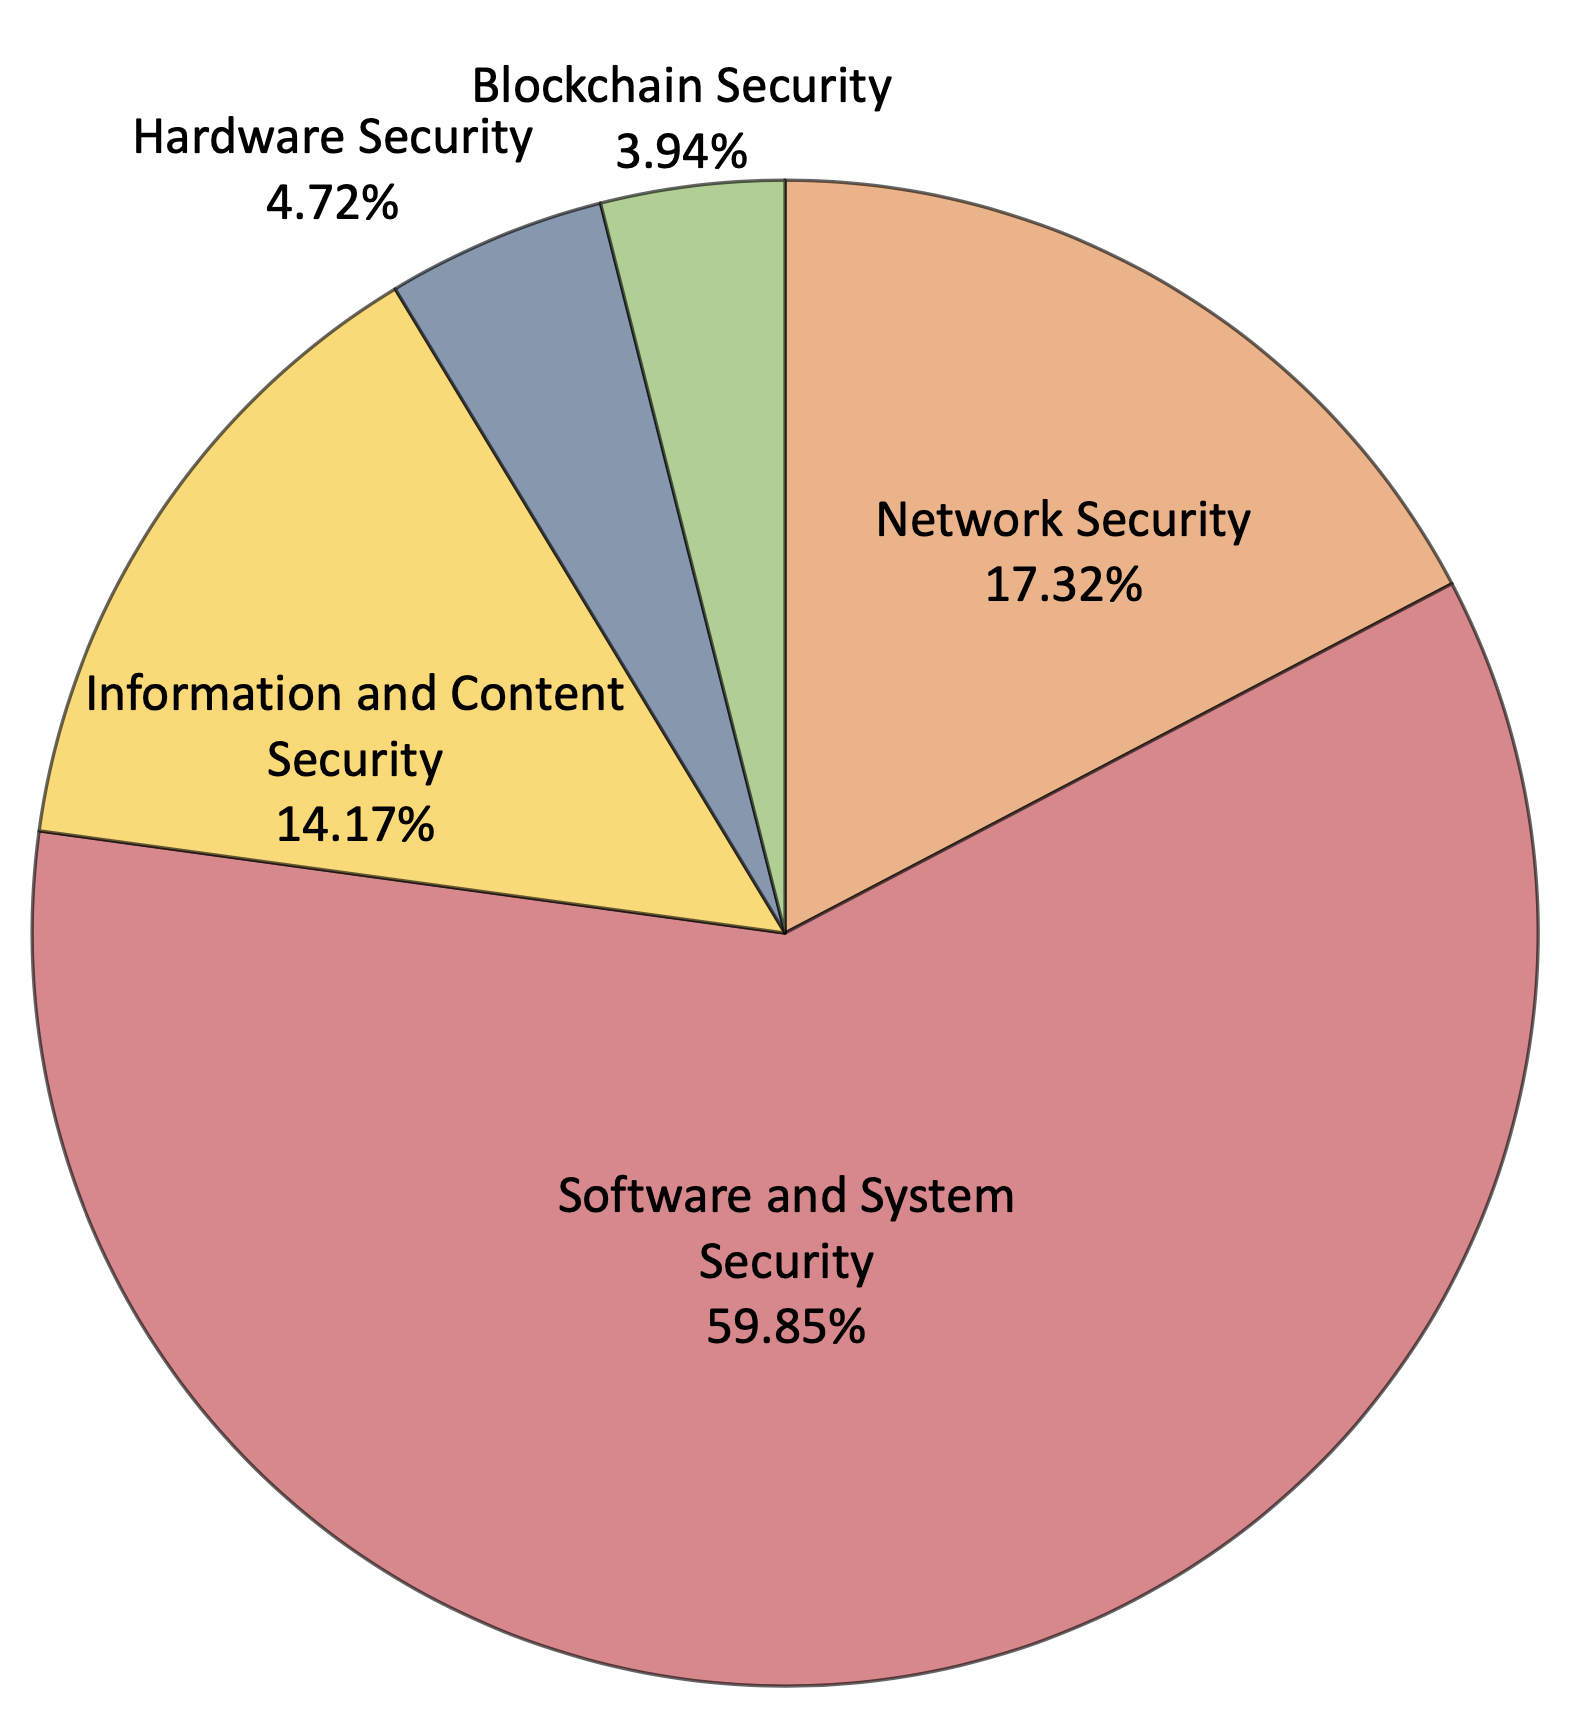
\includegraphics[width = 0.8\textwidth]{figures/Distribution of LLM usages in security domains}}}
                    \caption{Distribution of LLM usages in security domains \cite{citing4}}
                \end{figure}
            \subsubsection{Pratiques actuelles de développement par LLM : exemple d'IntelliCode}
                %45
    \section{Correction et complétion pendant la phase de développement : promesses et difficultés rencontrées}
        %50
    \section{Interprétation des métriques de classification présentées}
        %38
